\chapter{Approach}


% Describe the performed solution with all possible details. Define necessary parameters, inputs, outputs and context of use, possible problems and when they can be applied. 

% Remember to define necessary concepts before using them, building the text from easiest definitions (not depending on previous definitions) to complex definitions (depending on previous definitions).

% E.g: 
% \begin{itemize}
%	\item Lost Communication: a lost communication occurs when the conditions of the environment are not sufficient or the distance between sender and receiver is to hight to transmit information.
%	\item Wait until rescue: when the robot loses its communication, the pre-designed state machine will stop the motors to keep the actual position. Energy safe mode will be enabled, at the same time that a channel transceiver daemon will send SOS messages every T and wait for reply during T sec. 
%\end{itemize}

The challenge is how to coordinate multiple robots to execute a set of tasks. To tackele this problem, a communication efficient scheduler system is designed, where each robot autonomously request task from the centralized scheduler and centralized scheduler response with a set of suitable tasks. The architecture of this centralized scheduler is shown in Fig


\begin{figure}
	\centering
	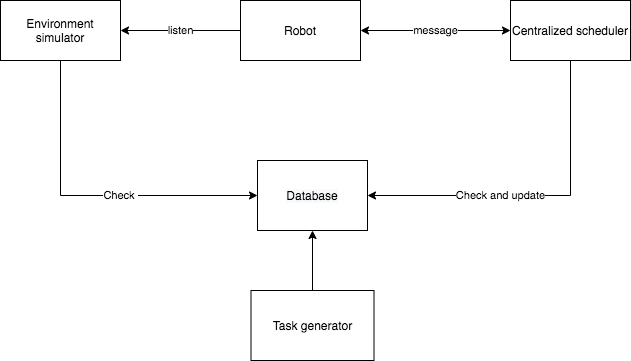
\includegraphics[width = 0.6\textwidth]{content/images/architecture.drawio.png}
	\caption{System architecture}
	\label{fig:system_architecture}
\end{figure}

\section{The System Parameters}

\item 
